% Created by tikzDevice version 0.12.3.1 on 2022-09-02 10:31:52
% !TEX encoding = UTF-8 Unicode
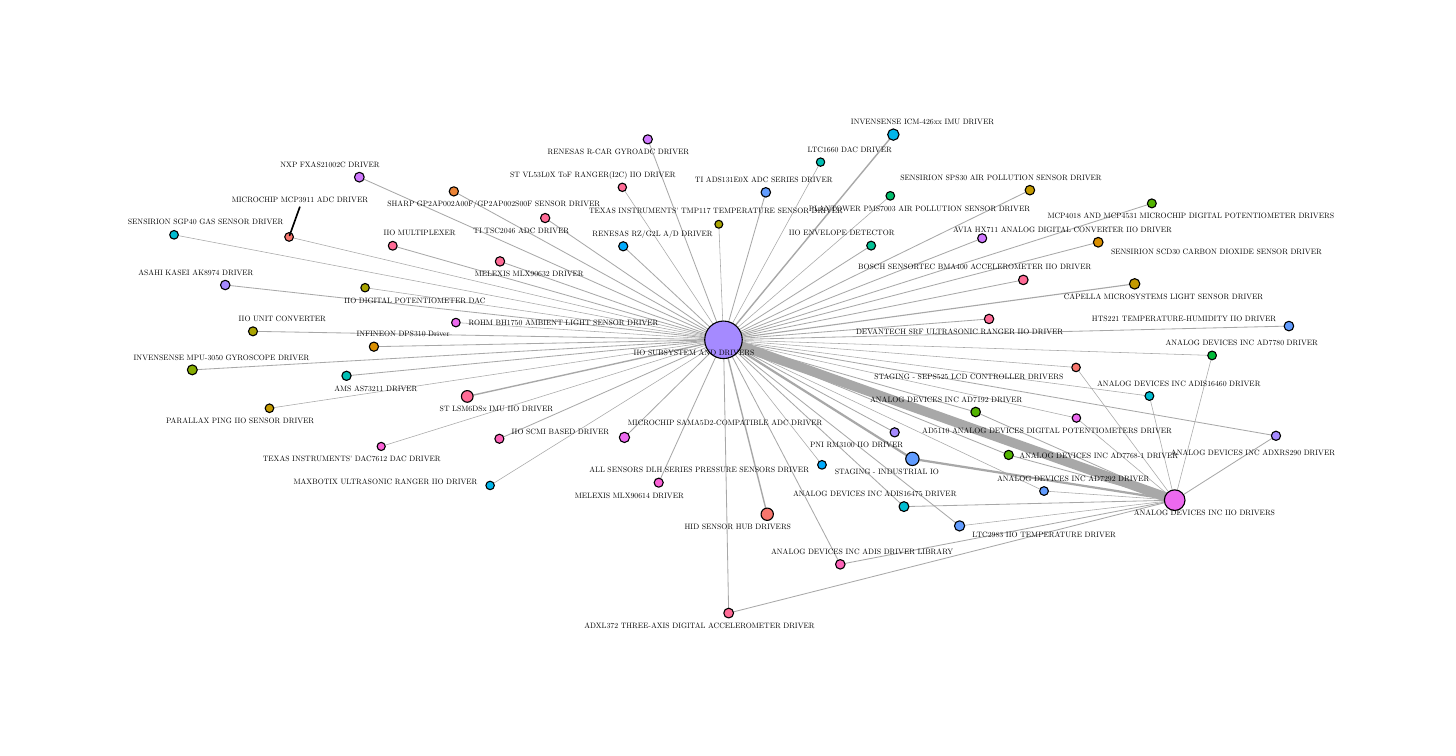
\begin{tikzpicture}[x=1pt,y=1pt]
\definecolor{fillColor}{RGB}{255,255,255}
\path[use as bounding box,fill=fillColor,fill opacity=0.00] (0,0) rectangle (505.89,252.94);
\begin{scope}
\path[clip] (  0.00,  0.00) rectangle (505.89,252.94);
\definecolor{fillColor}{RGB}{255,255,255}

\path[fill=fillColor] (  0.00,  0.00) rectangle (505.89,252.94);
\end{scope}
\begin{scope}
\path[clip] ( 32.75, 32.75) rectangle (475.89,222.94);
\definecolor{drawColor}{gray}{0.66}

\path[draw=drawColor,line width= 0.2pt,line join=round] (378.96,111.89) -- (414.47, 82.20);

\path[draw=drawColor,line width= 0.2pt,line join=round] (378.96,111.89) -- (251.43,140.15);

\path[draw=drawColor,line width= 0.3pt,line join=round] (253.30, 41.40) -- (414.47, 82.20);

\path[draw=drawColor,line width= 0.3pt,line join=round] (253.30, 41.40) -- (251.43,140.15);

\path[draw=drawColor,line width= 0.2pt,line join=round] (287.02, 94.97) -- (251.43,140.15);

\path[draw=drawColor,line width= 0.3pt,line join=round] (115.21,127.14) -- (251.43,140.15);

\path[draw=drawColor,line width= 0.3pt,line join=round] (342.55,114.06) -- (414.47, 82.20);

\path[draw=drawColor,line width= 0.3pt,line join=round] (342.55,114.06) -- (251.43,140.15);

\path[draw=drawColor,line width= 0.2pt,line join=round] (367.26, 85.50) -- (414.47, 82.20);

\path[draw=drawColor,line width= 0.2pt,line join=round] (367.26, 85.50) -- (251.43,140.15);

\path[draw=drawColor,line width= 0.3pt,line join=round] (354.48, 98.55) -- (414.47, 82.20);

\path[draw=drawColor,line width= 0.3pt,line join=round] (354.48, 98.55) -- (251.43,140.15);

\path[draw=drawColor,line width= 0.2pt,line join=round] (427.99,134.50) -- (414.47, 82.20);

\path[draw=drawColor,line width= 0.2pt,line join=round] (427.99,134.50) -- (251.43,140.15);

\path[draw=drawColor,line width= 0.3pt,line join=round] (293.63, 59.02) -- (414.47, 82.20);

\path[draw=drawColor,line width= 0.3pt,line join=round] (293.63, 59.02) -- (251.43,140.15);

\path[draw=drawColor,line width= 0.2pt,line join=round] (405.33,119.83) -- (414.47, 82.20);

\path[draw=drawColor,line width= 0.2pt,line join=round] (405.33,119.83) -- (251.43,140.15);

\path[draw=drawColor,line width= 0.3pt,line join=round] (316.64, 79.88) -- (414.47, 82.20);

\path[draw=drawColor,line width= 0.3pt,line join=round] (316.64, 79.88) -- (251.43,140.15);

\path[draw=drawColor,line width= 0.3pt,line join=round] (451.07,105.46) -- (414.47, 82.20);

\path[draw=drawColor,line width= 0.3pt,line join=round] (451.07,105.46) -- (251.43,140.15);

\path[draw=drawColor,line width= 3.4pt,line join=round] (414.47, 82.20) -- (251.43,140.15);

\path[draw=drawColor,line width= 0.2pt,line join=round] (414.47, 82.20) -- (336.74, 72.91);

\path[draw=drawColor,line width= 0.8pt,line join=round] (414.47, 82.20) -- (319.69, 97.13);

\path[draw=drawColor,line width= 0.2pt,line join=round] (414.47, 82.20) -- (378.82,130.16);

\path[draw=drawColor,line width= 0.3pt,line join=round] ( 71.39,159.95) -- (251.43,140.15);

\path[draw=drawColor,line width= 0.3pt,line join=round] (344.91,176.84) -- (251.43,140.15);

\path[draw=drawColor,line width= 0.3pt,line join=round] (359.77,161.79) -- (251.43,140.15);

\path[draw=drawColor,line width= 0.4pt,line join=round] (400.00,160.37) -- (251.43,140.15);

\path[draw=drawColor,line width= 0.3pt,line join=round] (347.39,147.68) -- (251.43,140.15);

\path[draw=drawColor,line width= 0.5pt,line join=round] (267.23, 77.12) -- (251.43,140.15);

\path[draw=drawColor,line width= 0.3pt,line join=round] (455.75,145.11) -- (251.43,140.15);

\path[draw=drawColor,line width= 0.2pt,line join=round] (121.92,158.98) -- (251.43,140.15);

\path[draw=drawColor,line width= 0.3pt,line join=round] (304.79,174.18) -- (251.43,140.15);

\path[draw=drawColor,line width= 0.3pt,line join=round] (131.91,174.13) -- (251.43,140.15);

\path[draw=drawColor,line width= 0.3pt,line join=round] (170.45,104.39) -- (251.43,140.15);

\path[draw=drawColor,line width= 0.3pt,line join=round] (251.43,140.15) -- ( 81.41,143.21);

\path[draw=drawColor,line width= 0.3pt,line join=round] (251.43,140.15) -- (125.11,137.67);

\path[draw=drawColor,line width= 0.5pt,line join=round] (251.43,140.15) -- (312.81,214.30);

\path[draw=drawColor,line width= 0.3pt,line join=round] (251.43,140.15) -- ( 59.49,129.28);

\path[draw=drawColor,line width= 0.2pt,line join=round] (251.43,140.15) -- (286.50,204.36);

\path[draw=drawColor,line width= 0.3pt,line join=round] (251.43,140.15) -- (336.74, 72.91);

\path[draw=drawColor,line width= 0.2pt,line join=round] (251.43,140.15) -- (167.10, 87.52);

\path[draw=drawColor,line width= 0.3pt,line join=round] (251.43,140.15) -- (406.21,189.44);

\path[draw=drawColor,line width= 0.3pt,line join=round] (251.43,140.15) -- (228.02, 88.53);

\path[draw=drawColor,line width= 0.3pt,line join=round] (251.43,140.15) -- (170.67,168.48);

\path[draw=drawColor,line width= 0.2pt,line join=round] (251.43,140.15) -- ( 94.46,177.32);

\path[draw=drawColor,line width= 0.3pt,line join=round] (251.43,140.15) -- (215.64,104.89);

\path[draw=drawColor,line width= 0.3pt,line join=round] (251.43,140.15) -- (119.85,198.92);

\path[draw=drawColor,line width= 0.2pt,line join=round] (251.43,140.15) -- ( 87.37,115.41);

\path[draw=drawColor,line width= 0.2pt,line join=round] (251.43,140.15) -- (311.71,192.17);

\path[draw=drawColor,line width= 0.3pt,line join=round] (251.43,140.15) -- (313.28,106.71);

\path[draw=drawColor,line width= 0.3pt,line join=round] (251.43,140.15) -- (224.07,212.58);

\path[draw=drawColor,line width= 0.3pt,line join=round] (251.43,140.15) -- (215.20,173.94);

\path[draw=drawColor,line width= 0.2pt,line join=round] (251.43,140.15) -- (154.73,146.38);

\path[draw=drawColor,line width= 0.3pt,line join=round] (251.43,140.15) -- (386.83,175.40);

\path[draw=drawColor,line width= 0.2pt,line join=round] (251.43,140.15) -- ( 52.89,178.09);

\path[draw=drawColor,line width= 0.3pt,line join=round] (251.43,140.15) -- (362.15,194.22);

\path[draw=drawColor,line width= 0.3pt,line join=round] (251.43,140.15) -- (153.99,193.78);

\path[draw=drawColor,line width= 0.5pt,line join=round] (251.43,140.15) -- (158.84,119.69);

\path[draw=drawColor,line width= 0.2pt,line join=round] (251.43,140.15) -- (214.88,195.25);

\path[draw=drawColor,line width= 0.8pt,line join=round] (251.43,140.15) -- (319.69, 97.13);

\path[draw=drawColor,line width= 0.2pt,line join=round] (251.43,140.15) -- (378.82,130.16);

\path[draw=drawColor,line width= 0.2pt,line join=round] (251.43,140.15) -- (127.74,101.62);

\path[draw=drawColor,line width= 0.2pt,line join=round] (251.43,140.15) -- (249.74,181.90);

\path[draw=drawColor,line width= 0.3pt,line join=round] (251.43,140.15) -- (266.72,193.44);

\path[draw=drawColor,line width= 0.3pt,line join=round] (251.43,140.15) -- (186.99,184.15);
\definecolor{drawColor}{RGB}{0,0,0}
\definecolor{fillColor}{RGB}{236,105,239}

\path[draw=drawColor,line width= 0.4pt,line join=round,line cap=round,fill=fillColor] (378.96,111.89) circle (  1.53);
\definecolor{fillColor}{RGB}{255,107,150}

\path[draw=drawColor,line width= 0.4pt,line join=round,line cap=round,fill=fillColor] (253.30, 41.40) circle (  1.77);
\definecolor{fillColor}{RGB}{0,171,253}

\path[draw=drawColor,line width= 0.4pt,line join=round,line cap=round,fill=fillColor] (287.02, 94.97) circle (  1.57);
\definecolor{fillColor}{RGB}{0,192,181}

\path[draw=drawColor,line width= 0.4pt,line join=round,line cap=round,fill=fillColor] (115.21,127.14) circle (  1.67);
\definecolor{fillColor}{RGB}{83,180,0}

\path[draw=drawColor,line width= 0.4pt,line join=round,line cap=round,fill=fillColor] (342.55,114.06) circle (  1.73);
\definecolor{fillColor}{RGB}{97,156,255}

\path[draw=drawColor,line width= 0.4pt,line join=round,line cap=round,fill=fillColor] (367.26, 85.50) circle (  1.58);
\definecolor{fillColor}{RGB}{83,180,0}

\path[draw=drawColor,line width= 0.4pt,line join=round,line cap=round,fill=fillColor] (354.48, 98.55) circle (  1.67);
\definecolor{fillColor}{RGB}{0,186,56}

\path[draw=drawColor,line width= 0.4pt,line join=round,line cap=round,fill=fillColor] (427.99,134.50) circle (  1.58);
\definecolor{fillColor}{RGB}{255,99,185}

\path[draw=drawColor,line width= 0.4pt,line join=round,line cap=round,fill=fillColor] (293.63, 59.02) circle (  1.72);
\definecolor{fillColor}{RGB}{0,189,210}

\path[draw=drawColor,line width= 0.4pt,line join=round,line cap=round,fill=fillColor] (405.33,119.83) circle (  1.59);

\path[draw=drawColor,line width= 0.4pt,line join=round,line cap=round,fill=fillColor] (316.64, 79.88) circle (  1.78);
\definecolor{fillColor}{RGB}{165,138,255}

\path[draw=drawColor,line width= 0.4pt,line join=round,line cap=round,fill=fillColor] (451.07,105.46) circle (  1.66);
\definecolor{fillColor}{RGB}{236,105,239}

\path[draw=drawColor,line width= 0.4pt,line join=round,line cap=round,fill=fillColor] (414.47, 82.20) circle (  3.73);
\definecolor{fillColor}{RGB}{165,138,255}

\path[draw=drawColor,line width= 0.4pt,line join=round,line cap=round,fill=fillColor] ( 71.39,159.95) circle (  1.71);
\definecolor{fillColor}{RGB}{208,120,255}

\path[draw=drawColor,line width= 0.4pt,line join=round,line cap=round,fill=fillColor] (344.91,176.84) circle (  1.64);
\definecolor{fillColor}{RGB}{255,107,150}

\path[draw=drawColor,line width= 0.4pt,line join=round,line cap=round,fill=fillColor] (359.77,161.79) circle (  1.73);
\definecolor{fillColor}{RGB}{196,154,0}

\path[draw=drawColor,line width= 0.4pt,line join=round,line cap=round,fill=fillColor] (400.00,160.37) circle (  1.88);
\definecolor{fillColor}{RGB}{255,107,150}

\path[draw=drawColor,line width= 0.4pt,line join=round,line cap=round,fill=fillColor] (347.39,147.68) circle (  1.70);
\definecolor{fillColor}{RGB}{248,118,109}

\path[draw=drawColor,line width= 0.4pt,line join=round,line cap=round,fill=fillColor] (267.23, 77.12) circle (  2.23);
\definecolor{fillColor}{RGB}{97,156,255}

\path[draw=drawColor,line width= 0.4pt,line join=round,line cap=round,fill=fillColor] (455.75,145.11) circle (  1.73);
\definecolor{fillColor}{RGB}{169,164,0}

\path[draw=drawColor,line width= 0.4pt,line join=round,line cap=round,fill=fillColor] (121.92,158.98) circle (  1.53);
\definecolor{fillColor}{RGB}{0,192,148}

\path[draw=drawColor,line width= 0.4pt,line join=round,line cap=round,fill=fillColor] (304.79,174.18) circle (  1.60);
\definecolor{fillColor}{RGB}{255,107,150}

\path[draw=drawColor,line width= 0.4pt,line join=round,line cap=round,fill=fillColor] (131.91,174.13) circle (  1.60);
\definecolor{fillColor}{RGB}{255,99,185}

\path[draw=drawColor,line width= 0.4pt,line join=round,line cap=round,fill=fillColor] (170.45,104.39) circle (  1.64);
\definecolor{fillColor}{RGB}{165,138,255}

\path[draw=drawColor,line width= 0.4pt,line join=round,line cap=round,fill=fillColor] (251.43,140.15) circle (  6.78);
\definecolor{fillColor}{RGB}{169,164,0}

\path[draw=drawColor,line width= 0.4pt,line join=round,line cap=round,fill=fillColor] ( 81.41,143.21) circle (  1.62);
\definecolor{fillColor}{RGB}{218,143,0}

\path[draw=drawColor,line width= 0.4pt,line join=round,line cap=round,fill=fillColor] (125.11,137.67) circle (  1.67);
\definecolor{fillColor}{RGB}{0,182,235}

\path[draw=drawColor,line width= 0.4pt,line join=round,line cap=round,fill=fillColor] (312.81,214.30) circle (  2.05);
\definecolor{fillColor}{RGB}{134,172,0}

\path[draw=drawColor,line width= 0.4pt,line join=round,line cap=round,fill=fillColor] ( 59.49,129.28) circle (  1.79);
\definecolor{fillColor}{RGB}{0,192,181}

\path[draw=drawColor,line width= 0.4pt,line join=round,line cap=round,fill=fillColor] (286.50,204.36) circle (  1.51);
\definecolor{fillColor}{RGB}{97,156,255}

\path[draw=drawColor,line width= 0.4pt,line join=round,line cap=round,fill=fillColor] (336.74, 72.91) circle (  1.85);
\definecolor{fillColor}{RGB}{0,182,235}

\path[draw=drawColor,line width= 0.4pt,line join=round,line cap=round,fill=fillColor] (167.10, 87.52) circle (  1.53);
\definecolor{fillColor}{RGB}{83,180,0}

\path[draw=drawColor,line width= 0.4pt,line join=round,line cap=round,fill=fillColor] (406.21,189.44) circle (  1.61);
\definecolor{fillColor}{RGB}{251,97,215}

\path[draw=drawColor,line width= 0.4pt,line join=round,line cap=round,fill=fillColor] (228.02, 88.53) circle (  1.64);
\definecolor{fillColor}{RGB}{255,107,150}

\path[draw=drawColor,line width= 0.4pt,line join=round,line cap=round,fill=fillColor] (170.67,168.48) circle (  1.70);
\definecolor{fillColor}{RGB}{248,118,109}

\path[draw=drawColor,line width= 0.4pt,line join=round,line cap=round,fill=fillColor] ( 94.46,177.32) circle (  1.57);
\definecolor{fillColor}{RGB}{236,105,239}

\path[draw=drawColor,line width= 0.4pt,line join=round,line cap=round,fill=fillColor] (215.64,104.89) circle (  1.85);
\definecolor{fillColor}{RGB}{208,120,255}

\path[draw=drawColor,line width= 0.4pt,line join=round,line cap=round,fill=fillColor] (119.85,198.92) circle (  1.76);
\definecolor{fillColor}{RGB}{196,154,0}

\path[draw=drawColor,line width= 0.4pt,line join=round,line cap=round,fill=fillColor] ( 87.37,115.41) circle (  1.55);
\definecolor{fillColor}{RGB}{0,190,109}

\path[draw=drawColor,line width= 0.4pt,line join=round,line cap=round,fill=fillColor] (311.71,192.17) circle (  1.56);
\definecolor{fillColor}{RGB}{165,138,255}

\path[draw=drawColor,line width= 0.4pt,line join=round,line cap=round,fill=fillColor] (313.28,106.71) circle (  1.66);
\definecolor{fillColor}{RGB}{208,120,255}

\path[draw=drawColor,line width= 0.4pt,line join=round,line cap=round,fill=fillColor] (224.07,212.58) circle (  1.66);
\definecolor{fillColor}{RGB}{0,171,253}

\path[draw=drawColor,line width= 0.4pt,line join=round,line cap=round,fill=fillColor] (215.20,173.94) circle (  1.65);
\definecolor{fillColor}{RGB}{236,105,239}

\path[draw=drawColor,line width= 0.4pt,line join=round,line cap=round,fill=fillColor] (154.73,146.38) circle (  1.55);
\definecolor{fillColor}{RGB}{218,143,0}

\path[draw=drawColor,line width= 0.4pt,line join=round,line cap=round,fill=fillColor] (386.83,175.40) circle (  1.75);
\definecolor{fillColor}{RGB}{0,189,210}

\path[draw=drawColor,line width= 0.4pt,line join=round,line cap=round,fill=fillColor] ( 52.89,178.09) circle (  1.56);
\definecolor{fillColor}{RGB}{196,154,0}

\path[draw=drawColor,line width= 0.4pt,line join=round,line cap=round,fill=fillColor] (362.15,194.22) circle (  1.72);
\definecolor{fillColor}{RGB}{235,131,53}

\path[draw=drawColor,line width= 0.4pt,line join=round,line cap=round,fill=fillColor] (153.99,193.78) circle (  1.67);
\definecolor{fillColor}{RGB}{255,107,150}

\path[draw=drawColor,line width= 0.4pt,line join=round,line cap=round,fill=fillColor] (158.84,119.69) circle (  2.11);

\path[draw=drawColor,line width= 0.4pt,line join=round,line cap=round,fill=fillColor] (214.88,195.25) circle (  1.51);
\definecolor{fillColor}{RGB}{97,156,255}

\path[draw=drawColor,line width= 0.4pt,line join=round,line cap=round,fill=fillColor] (319.69, 97.13) circle (  2.41);
\definecolor{fillColor}{RGB}{248,118,109}

\path[draw=drawColor,line width= 0.4pt,line join=round,line cap=round,fill=fillColor] (378.82,130.16) circle (  1.54);
\definecolor{fillColor}{RGB}{251,97,215}

\path[draw=drawColor,line width= 0.4pt,line join=round,line cap=round,fill=fillColor] (127.74,101.62) circle (  1.47);
\definecolor{fillColor}{RGB}{169,164,0}

\path[draw=drawColor,line width= 0.4pt,line join=round,line cap=round,fill=fillColor] (249.74,181.90) circle (  1.43);
\definecolor{fillColor}{RGB}{97,156,255}

\path[draw=drawColor,line width= 0.4pt,line join=round,line cap=round,fill=fillColor] (266.72,193.44) circle (  1.72);
\definecolor{fillColor}{RGB}{255,107,150}

\path[draw=drawColor,line width= 0.4pt,line join=round,line cap=round,fill=fillColor] (186.99,184.15) circle (  1.67);

\path[draw=drawColor,line width= 0.6pt,line join=round,line cap=round] ( 98.32,188.11) -- ( 94.65,177.86);

\node[text=drawColor,anchor=base,inner sep=0pt, outer sep=0pt, scale=  0.28] at (368.34,106.31) {AD5110 ANALOG DEVICES DIGITAL POTENTIOMETERS DRIVER};

\node[text=drawColor,anchor=base,inner sep=0pt, outer sep=0pt, scale=  0.28] at (242.76, 35.88) {ADXL372 THREE-AXIS DIGITAL ACCELEROMETER DRIVER};

\node[text=drawColor,anchor=base,inner sep=0pt, outer sep=0pt, scale=  0.28] at (242.65, 92.13) {ALL SENSORS DLH SERIES PRESSURE SENSORS DRIVER};

\node[text=drawColor,anchor=base,inner sep=0pt, outer sep=0pt, scale=  0.28] at (125.81,121.60) {AMS AS73211 DRIVER};

\node[text=drawColor,anchor=base,inner sep=0pt, outer sep=0pt, scale=  0.28] at (331.94,117.61) {ANALOG DEVICES INC AD7192 DRIVER};

\node[text=drawColor,anchor=base,inner sep=0pt, outer sep=0pt, scale=  0.28] at (377.82, 89.07) {ANALOG DEVICES INC AD7292 DRIVER};

\node[text=drawColor,anchor=base,inner sep=0pt, outer sep=0pt, scale=  0.28] at (387.00, 97.16) {ANALOG DEVICES INC AD7768-1 DRIVER};

\node[text=drawColor,anchor=base,inner sep=0pt, outer sep=0pt, scale=  0.28] at (438.71,138.12) {ANALOG DEVICES INC AD7780 DRIVER};

\node[text=drawColor,anchor=base,inner sep=0pt, outer sep=0pt, scale=  0.28] at (301.52, 62.58) {ANALOG DEVICES INC ADIS DRIVER LIBRARY};

\node[text=drawColor,anchor=base,inner sep=0pt, outer sep=0pt, scale=  0.28] at (415.96,123.39) {ANALOG DEVICES INC ADIS16460 DRIVER};

\node[text=drawColor,anchor=base,inner sep=0pt, outer sep=0pt, scale=  0.28] at (306.11, 83.44) {ANALOG DEVICES INC ADIS16475 DRIVER};

\node[text=drawColor,anchor=base,inner sep=0pt, outer sep=0pt, scale=  0.28] at (442.77, 98.35) {ANALOG DEVICES INC ADXRS290 DRIVER};

\node[text=drawColor,anchor=base,inner sep=0pt, outer sep=0pt, scale=  0.28] at (425.21, 76.66) {ANALOG DEVICES INC IIO DRIVERS};

\node[text=drawColor,anchor=base,inner sep=0pt, outer sep=0pt, scale=  0.28] at ( 60.78,163.54) {ASAHI KASEI AK8974 DRIVER};

\node[text=drawColor,anchor=base,inner sep=0pt, outer sep=0pt, scale=  0.28] at (373.92,178.99) {AVIA HX711 ANALOG DIGITAL CONVERTER IIO DRIVER};

\node[text=drawColor,anchor=base,inner sep=0pt, outer sep=0pt, scale=  0.28] at (342.20,165.38) {BOSCH SENSORTEC BMA400 ACCELEROMETER IIO DRIVER};

\node[text=drawColor,anchor=base,inner sep=0pt, outer sep=0pt, scale=  0.28] at (410.43,154.88) {CAPELLA MICROSYSTEMS LIGHT SENSOR DRIVER};

\node[text=drawColor,anchor=base,inner sep=0pt, outer sep=0pt, scale=  0.28] at (336.76,142.12) {DEVANTECH SRF ULTRASONIC RANGER IIO DRIVER};

\node[text=drawColor,anchor=base,inner sep=0pt, outer sep=0pt, scale=  0.28] at (256.62, 71.60) {HID SENSOR HUB DRIVERS};

\node[text=drawColor,anchor=base,inner sep=0pt, outer sep=0pt, scale=  0.28] at (417.86,146.75) {HTS221 TEMPERATURE-HUMIDITY IIO DRIVER};

\node[text=drawColor,anchor=base,inner sep=0pt, outer sep=0pt, scale=  0.28] at (139.95,153.45) {IIO DIGITAL POTENTIOMETER DAC};

\node[text=drawColor,anchor=base,inner sep=0pt, outer sep=0pt, scale=  0.28] at (294.15,177.78) {IIO ENVELOPE DETECTOR};

\node[text=drawColor,anchor=base,inner sep=0pt, outer sep=0pt, scale=  0.28] at (141.63,177.72) {IIO MULTIPLEXER};

\node[text=drawColor,anchor=base,inner sep=0pt, outer sep=0pt, scale=  0.28] at (192.51,106.08) {IIO SCMI BASED DRIVER};

\node[text=drawColor,anchor=base,inner sep=0pt, outer sep=0pt, scale=  0.28] at (240.78,134.61) {IIO SUBSYSTEM AND DRIVERS};

\node[text=drawColor,anchor=base,inner sep=0pt, outer sep=0pt, scale=  0.28] at ( 92.01,146.78) {IIO UNIT CONVERTER};

\node[text=drawColor,anchor=base,inner sep=0pt, outer sep=0pt, scale=  0.28] at (135.66,141.22) {INFINEON DPS310 Driver};

\node[text=drawColor,anchor=base,inner sep=0pt, outer sep=0pt, scale=  0.28] at (323.35,217.87) {INVENSENSE ICM-426xx IMU DRIVER};

\node[text=drawColor,anchor=base,inner sep=0pt, outer sep=0pt, scale=  0.28] at ( 70.03,132.84) {INVENSENSE MPU-3050 GYROSCOPE DRIVER};

\node[text=drawColor,anchor=base,inner sep=0pt, outer sep=0pt, scale=  0.28] at (297.04,207.92) {LTC1660 DAC DRIVER};

\node[text=drawColor,anchor=base,inner sep=0pt, outer sep=0pt, scale=  0.28] at (367.30, 68.65) {LTC2983 IIO TEMPERATURE DRIVER};

\node[text=drawColor,anchor=base,inner sep=0pt, outer sep=0pt, scale=  0.28] at (129.30, 88.04) {MAXBOTIX ULTRASONIC RANGER IIO DRIVER};

\node[text=drawColor,anchor=base,inner sep=0pt, outer sep=0pt, scale=  0.28] at (420.29,183.90) {MCP4018 AND MCP4531 MICROCHIP DIGITAL POTENTIOMETER DRIVERS};

\node[text=drawColor,anchor=base,inner sep=0pt, outer sep=0pt, scale=  0.28] at (217.40, 82.98) {MELEXIS MLX90614 DRIVER};

\node[text=drawColor,anchor=base,inner sep=0pt, outer sep=0pt, scale=  0.28] at (181.23,162.94) {MELEXIS MLX90632 DRIVER};

\node[text=drawColor,anchor=base,inner sep=0pt, outer sep=0pt, scale=  0.28] at ( 98.37,189.62) {MICROCHIP MCP3911 ADC DRIVER};

\node[text=drawColor,anchor=base,inner sep=0pt, outer sep=0pt, scale=  0.28] at (252.03,109.17) {MICROCHIP SAMA5D2-COMPATIBLE ADC DRIVER};

\node[text=drawColor,anchor=base,inner sep=0pt, outer sep=0pt, scale=  0.28] at (109.25,202.49) {NXP FXAS21002C DRIVER};

\node[text=drawColor,anchor=base,inner sep=0pt, outer sep=0pt, scale=  0.28] at ( 76.77,109.89) {PARALLAX PING IIO SENSOR DRIVER};

\node[text=drawColor,anchor=base,inner sep=0pt, outer sep=0pt, scale=  0.28] at (322.24,186.66) {PLANTOWER PMS7003 AIR POLLUTION SENSOR DRIVER};

\node[text=drawColor,anchor=base,inner sep=0pt, outer sep=0pt, scale=  0.28] at (299.51,101.17) {PNI RM3100 IIO DRIVER};

\node[text=drawColor,anchor=base,inner sep=0pt, outer sep=0pt, scale=  0.28] at (213.46,207.03) {RENESAS R-CAR GYROADC DRIVER};

\node[text=drawColor,anchor=base,inner sep=0pt, outer sep=0pt, scale=  0.28] at (225.79,177.50) {RENESAS RZ/G2L A/D DRIVER};

\node[text=drawColor,anchor=base,inner sep=0pt, outer sep=0pt, scale=  0.28] at (193.63,145.46) {ROHM BH1750 AMBIENT LIGHT SENSOR DRIVER};

\node[text=drawColor,anchor=base,inner sep=0pt, outer sep=0pt, scale=  0.28] at (429.55,170.99) {SENSIRION SCD30 CARBON DIOXIDE SENSOR DRIVER};

\node[text=drawColor,anchor=base,inner sep=0pt, outer sep=0pt, scale=  0.28] at ( 64.30,181.66) {SENSIRION SGP40 GAS SENSOR DRIVER};

\node[text=drawColor,anchor=base,inner sep=0pt, outer sep=0pt, scale=  0.28] at (351.69,197.77) {SENSIRION SPS30 AIR POLLUTION SENSOR DRIVER};

\node[text=drawColor,anchor=base,inner sep=0pt, outer sep=0pt, scale=  0.28] at (168.42,188.25) {SHARP GP2AP002A00F/GP2AP002S00F SENSOR DRIVER};

\node[text=drawColor,anchor=base,inner sep=0pt, outer sep=0pt, scale=  0.28] at (169.39,114.19) {ST LSM6DSx IMU IIO DRIVER};

\node[text=drawColor,anchor=base,inner sep=0pt, outer sep=0pt, scale=  0.28] at (204.22,198.81) {ST VL53L0X ToF RANGER(I2C) IIO DRIVER};

\node[text=drawColor,anchor=base,inner sep=0pt, outer sep=0pt, scale=  0.28] at (310.47, 91.58) {STAGING - INDUSTRIAL IO};

\node[text=drawColor,anchor=base,inner sep=0pt, outer sep=0pt, scale=  0.28] at (340.09,125.67) {STAGING - SEPS525 LCD CONTROLLER DRIVERS};

\node[text=drawColor,anchor=base,inner sep=0pt, outer sep=0pt, scale=  0.28] at (117.09, 96.06) {TEXAS INSTRUMENTS' DAC7612 DAC DRIVER};

\node[text=drawColor,anchor=base,inner sep=0pt, outer sep=0pt, scale=  0.28] at (248.70,185.77) {TEXAS INSTRUMENTS' TMP117 TEMPERATURE SENSOR DRIVER};

\node[text=drawColor,anchor=base,inner sep=0pt, outer sep=0pt, scale=  0.28] at (265.98,197.06) {TI ADS131E0X ADC SERIES DRIVER};

\node[text=drawColor,anchor=base,inner sep=0pt, outer sep=0pt, scale=  0.28] at (178.38,178.60) {TI TSC2046 ADC DRIVER};
\end{scope}
\end{tikzpicture}
